% !TeX root = ../mthesis.tex
% !TeX encoding = UTF-8
% !TeX spellcheck = en_US


%% == LaTeX ============================================================= %%
%% https://en.wikibooks.org/wiki/LaTeX
%% ====================================================================== %%


%% -- 2.4 Colors -------------------------------------------------------- %%
%% https://en.wikibooks.org/wiki/LaTeX/Colors
\usepackage[usenames,dvipsnames,svgnames,table]{xcolor}
\input{PREAMBLE/Colors.tex}
%% ---------------------------------------------------------------------- %%


%% -- 2.8 Internationalization ------------------------------------------ %%
%% https://en.wikibooks.org/wiki/LaTeX/Internationalization
\usepackage[utf8x]{inputenc} 		% input
\usepackage[LGR,T1]{fontenc}	 	% output (PDF)
\usepackage[english]{babel}			% language

%% ---------------------------------------------------------------------- %%


%% -- 2.10 Tables ------------------------------------------------------- %%
% https://en.wikibooks.org/wiki/LaTeX/Tables
%% ---------------------------------------------------------------------- %%


%% -- 2.16-17 Hyperlinks ------------------------------------------------ %%
% https://en.wikibooks.org/wiki/LaTeX/Hyperlinks
% https://en.wikibooks.org/wiki/LaTeX/Labels_and_Cross-referencing
\usepackage{hyperref}
%\usepackage[xindy,toc]{glossaries}
\usepackage[toc]{glossaries}
\usepackage[]{index}
%% ---------------------------------------------------------------------- %%


%% -- 4.1-3 Mathematics ------------------------------------------------- %%
% https://en.wikibooks.org/wiki/LaTeX/Mathematics
% https://en.wikibooks.org/wiki/LaTeX/Advanced_Mathematics
\usepackage{amsmath}
\usepackage{mathtools}
\usepackage{amssymb}

% https://en.wikibooks.org/wiki/LaTeX/Theorems
\usepackage{amsthm}
\usepackage{proof}
\usepackage{bussproofs}
\usepackage{marvosym}

\usepackage{multirow}
\usepackage[makeroom]{cancel} % \(b|x)cancel(to{}){}
\usepackage{soul}
\usepackage{pdfcomment}


%% ---------------------------------------------------------------------- %%


\usepackage{varioref}


%\usepackage{calc}
%\usepackage{geometry}

%% -- 4.5 Algorithms ---------------------------------------------------- %%
% https://en.wikibooks.org/wiki/LaTeX/Algorithms
%% ---------------------------------------------------------------------- %%


%% -- 4.6 Listings ------------------------------------------------------ %%
% https://en.wikibooks.org/wiki/LaTeX/Source_Code_Listings
\usepackage{listings}
\input{PREAMBLE/Listings.tex}	% definitions
%% ---------------------------------------------------------------------- %%


%% -- Graphics ---------------------------------------------------------- %%
% https://en.wikibooks.org/wiki/LaTeX/PGF/TikZ
\usepackage{tikz}
\documentclass{clseminar}

    \usepackage{tikz}

    % \documentclass{clseminar}

    \usepackage{tikz}

    % \documentclass{clseminar}

    \usepackage{tikz}

    % \input{../PREAMBLE/Drawings}

\begin{document}

\begin{figure}
\input{../DRAWINGS/ProperOrder}
\caption{Proper orders on terms}
\end{figure}

\begin{figure}
\input{../DRAWINGS/PartialOrder}
\end{figure}

\end{document}

\begin{document}

\begin{figure}
\begin{tikzpicture}
    \node (defCUC) at (-4,8.5) { $s\succ t\Rightarrow C[s]\succ C[t]$};
    \node (CUC) at (-4,8) { contexts };
    \node (defCUS) at (0,8.5) { $s\succ t\Rightarrow s\sigma\succ t\sigma$};
    \node (CUS) at (0,8) { substitutions };

        \node (CL) at (-2,6) { closed under };
        \node (defIRR) at (2,6.5) { $s\not>s$ };
        \node (IRR) at (6,6) { irreflexive };
        \node (defIRR) at (6,6.5) { $s>t>u\Rightarrow s>u$ };
        \node (TRA) at (2,6) { transitive };

        \node (PO) at (4,4.4) { $>$ };
        \node (PO) at (4,4) { proper order };
        \node (RWR) at (0,4) { rewrite relation };

        \node (defSTP) at (-2,2.5) { $C[s]\succ s$ };
        \node (STP) at (-2,2) { subterm property };
        \node (RWO) at (2,2) { rewrite order };
        \node (defWF) at (8,4.5) { $(s_i Rs_{i+1})_i$ is finite };
        \node (WF) at (8,4) { well-founded };

        \node (SO) at (0,0) {simplification order};
        \node (RO) at (4,0) {reduction order};

        \node (WFO) at (6,2) { well-founded order };


        \draw[->] (CL) -- (CUC);
        \draw[->] (CL) -- (CUS);

        \draw[->] (PO) -- (IRR);
        \draw[->] (PO) -- (TRA);π

        \draw[->] (RWR) -- (CL);

        \draw[->] (RWO) -- (PO);
        \draw[->] (RWO) -- (RWR);

        \draw[->] (SO) -- (STP);
        \draw[->] (RO) -- (RWO);
        \draw[->] (RO) -- (WFO);
        % \draw (RO) edge[out=0,in=-45,->] (WF);

        \draw[->] (SO) -- (RWO);
        \draw[->, dotted] (SO) -- (RO);

        \draw[->] (WFO) -- (WF);
        \draw[->] (WFO) -- (PO);

        \draw[->, dotted] (WF) -- (IRR);


    \end{tikzpicture}
\caption{Proper orders on terms}
\end{figure}

\begin{figure}
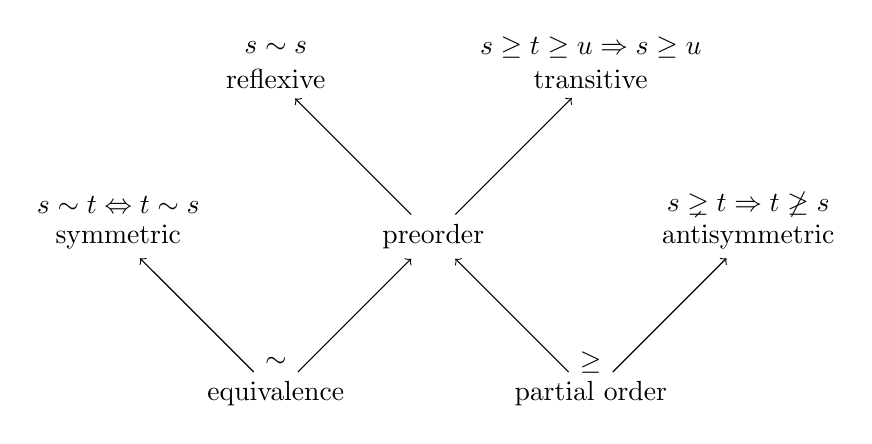
\begin{tikzpicture}

        \node (defSYMMETRIC) at (-4,0.4) { \( s\sim t\Leftrightarrow t\sim s \) };
        \node (SYMMETRIC) at (-4,0) { symmetric };

            \node (defREFLEXIVE) at (-2,2.4) { \( s\sim s \) };
            \node (REFLEXIVE) at (-2,2) { reflexive };

                \node (defTRANSITIVE) at (2,2.4) { \( s\geq t\geq u\Rightarrow s\geq u \) };
                \node (TRANSITIVE) at (2,2) { transitive };

                    \node (defANTISYMMETRIC) at (4,0.4) { \( s\gneq t \Rightarrow t\not\geq s \) };
                    \node (ANTISYMMETRIC) at (4,0) { antisymmetric };

        \node (PREORDER) at (0,0) { preorder };

    \node (SIM) at (-2,-1.6) { \( \sim \) };
    \node (EQUIVALENCE) at (-2,-2) { equivalence };

    \node (GEQ) at (2,-1.6) { \( \geq \) };
    \node (PARTIAL) at (2,-2) { partial order };

    % \node (PROPER) at (5,-1.5) { proper order };

    \draw[->] (PREORDER) -- (REFLEXIVE);
    \draw[->] (PREORDER) -- (TRANSITIVE);

    \draw[->] (EQUIVALENCE) -- (SYMMETRIC);
    \draw[->] (EQUIVALENCE) -- (PREORDER);
    \draw[->] (PARTIAL) -- (PREORDER);
    \draw[->] (PARTIAL) -- (ANTISYMMETRIC);

    % \draw[->] (PROPER) -- (TRANSITIVE);
\end{tikzpicture}
\end{figure}

\end{document}

\begin{document}

\begin{figure}
\begin{tikzpicture}
    \node (defCUC) at (-4,8.5) { $s\succ t\Rightarrow C[s]\succ C[t]$};
    \node (CUC) at (-4,8) { contexts };
    \node (defCUS) at (0,8.5) { $s\succ t\Rightarrow s\sigma\succ t\sigma$};
    \node (CUS) at (0,8) { substitutions };

        \node (CL) at (-2,6) { closed under };
        \node (defIRR) at (2,6.5) { $s\not>s$ };
        \node (IRR) at (6,6) { irreflexive };
        \node (defIRR) at (6,6.5) { $s>t>u\Rightarrow s>u$ };
        \node (TRA) at (2,6) { transitive };

        \node (PO) at (4,4.4) { $>$ };
        \node (PO) at (4,4) { proper order };
        \node (RWR) at (0,4) { rewrite relation };

        \node (defSTP) at (-2,2.5) { $C[s]\succ s$ };
        \node (STP) at (-2,2) { subterm property };
        \node (RWO) at (2,2) { rewrite order };
        \node (defWF) at (8,4.5) { $(s_i Rs_{i+1})_i$ is finite };
        \node (WF) at (8,4) { well-founded };

        \node (SO) at (0,0) {simplification order};
        \node (RO) at (4,0) {reduction order};

        \node (WFO) at (6,2) { well-founded order };


        \draw[->] (CL) -- (CUC);
        \draw[->] (CL) -- (CUS);

        \draw[->] (PO) -- (IRR);
        \draw[->] (PO) -- (TRA);π

        \draw[->] (RWR) -- (CL);

        \draw[->] (RWO) -- (PO);
        \draw[->] (RWO) -- (RWR);

        \draw[->] (SO) -- (STP);
        \draw[->] (RO) -- (RWO);
        \draw[->] (RO) -- (WFO);
        % \draw (RO) edge[out=0,in=-45,->] (WF);

        \draw[->] (SO) -- (RWO);
        \draw[->, dotted] (SO) -- (RO);

        \draw[->] (WFO) -- (WF);
        \draw[->] (WFO) -- (PO);

        \draw[->, dotted] (WF) -- (IRR);


    \end{tikzpicture}
\caption{Proper orders on terms}
\end{figure}

\begin{figure}
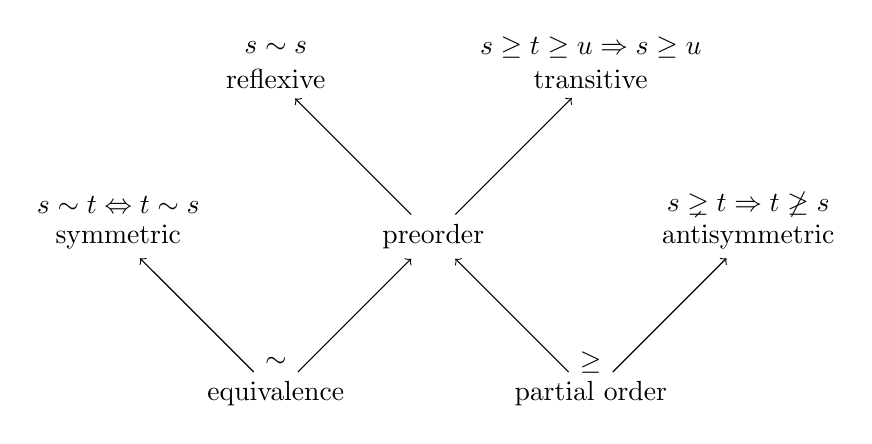
\begin{tikzpicture}

        \node (defSYMMETRIC) at (-4,0.4) { \( s\sim t\Leftrightarrow t\sim s \) };
        \node (SYMMETRIC) at (-4,0) { symmetric };

            \node (defREFLEXIVE) at (-2,2.4) { \( s\sim s \) };
            \node (REFLEXIVE) at (-2,2) { reflexive };

                \node (defTRANSITIVE) at (2,2.4) { \( s\geq t\geq u\Rightarrow s\geq u \) };
                \node (TRANSITIVE) at (2,2) { transitive };

                    \node (defANTISYMMETRIC) at (4,0.4) { \( s\gneq t \Rightarrow t\not\geq s \) };
                    \node (ANTISYMMETRIC) at (4,0) { antisymmetric };

        \node (PREORDER) at (0,0) { preorder };

    \node (SIM) at (-2,-1.6) { \( \sim \) };
    \node (EQUIVALENCE) at (-2,-2) { equivalence };

    \node (GEQ) at (2,-1.6) { \( \geq \) };
    \node (PARTIAL) at (2,-2) { partial order };

    % \node (PROPER) at (5,-1.5) { proper order };

    \draw[->] (PREORDER) -- (REFLEXIVE);
    \draw[->] (PREORDER) -- (TRANSITIVE);

    \draw[->] (EQUIVALENCE) -- (SYMMETRIC);
    \draw[->] (EQUIVALENCE) -- (PREORDER);
    \draw[->] (PARTIAL) -- (PREORDER);
    \draw[->] (PARTIAL) -- (ANTISYMMETRIC);

    % \draw[->] (PROPER) -- (TRANSITIVE);
\end{tikzpicture}
\end{figure}

\end{document}		% definitions and tikz macros
\usepackage[thinlines,thiklines]{easybmat}
%% ---------------------------------------------------------------------- %%

%% -- Macros ------------------------------------------------------------ %%
%% https://en.wikibooks.org/wiki/LaTeX/Macros
\usepackage{xspace}
% !TeX encoding = UTF-8

%% ==============================================================
%% ### MY MATH ENVIRONMENTS ###

\theoremstyle{plain}
%\newtheorem{theorem}{Theorem}			% predefined in CL?
%\newtheorem{proposition}{Proposition}	% predefined in CL?
%\newtheorem{lemma}{Lemma}				% predefined in CL?
%\newtheorem*{corollary}{Corollary}		% predefined in CL?

\theoremstyle{definition}
%\newtheorem{definition}{Definition}	% predefined in CL?
\newtheorem{conjecture}{Conjecture}
%\newtheorem*{example}{Example}			% predefined in CL?
%\newtheorem{algorithm}{Algorithm}		% predefined in CL
\newtheorem{procedure}{Procedure}
\newtheorem{goal}{Goal}
\newtheorem{notation}{Notation}

\theoremstyle{remark}
\newtheorem*{remark}{Remark}			% predefined in CL?
\newtheorem*{observation}{Observation}
%\newtheorem*{note}{Note}
%\newtheorem{case}{Case}

%% ==============================================================
%% ### MY MATH DEFINITIONS ###

% math alphabets

\DeclareMathAlphabet{\mathpzc}{OT1}{pzc}{m}{it}	% \mathpzc
\DeclareMathAlphabet{\mathcll}{T1}{calligra}{m}{n}

% math operators

\DeclareMathOperator{\arity}{arity}		% arity of a symbol

\DeclareMathOperator{\var}{\mathpzc{Vars}}			% variables of a term
\DeclareMathOperator{\fun}{\mathpzc{Funs}}			% function symbols of a term
\DeclareMathOperator{\pos}{\mathpzc{Pos}}			% positions in a term
\DeclareMathOperator{\posT}{\mathpzc{{t-}Pos}}			% positions in a term
\DeclareMathOperator{\posS}{\mathpzc{Pos^F}}
\DeclareMathOperator{\fvar}{\mathpzc{Fvars}}
\DeclareMathOperator{\bvar}{\mathpzc{Bvars}}

\DeclareMathOperator{\domain}{dom}			% domain of an assignment
\DeclareMathOperator{\range}{rng}		% range of an assignment
\DeclareMathOperator{\image}{img}			% image of an assignment

\DeclareMathOperator{\mgu}{mgu}			% most general unifier
\DeclareMathOperator{\sel}{sel}			% selection function

%\DeclareMathOperator{\mul}{mul}
%\DeclareMathOperator{\add}{add}
\DeclareMathOperator{\head}{head}
\DeclareMathOperator{\tail}{tail}
\DeclareMathOperator{\length}{length}



\DeclareMathOperator{\UNIF}{unifiable}
\DeclareMathOperator{\INST}{instance}
\DeclareMathOperator{\GNRL}{generalization}
\DeclareMathOperator{\VRNT}{variant}
\DeclareMathOperator{\PSTR}{pstr}

%\DeclareMathOperator{\subterms}{\mathpzc{Subterms}}	
%\DeclareMathOperator{\termsize}{size}
%\DeclareMathOperator{\symbols}{symbols}
%\DeclareMathOperator{\subforms}{\mathpzc{Subforms}}	
% !TeX encoding = UTF-8

% shortens the definition by cases
\newcommand{\DEFINE}[3][=]{{
		\begin{gather*}
		#2 #1 \left \{
				\begin{array}{ll}
					#3
				\end{array}
		\right.
		\end{gather*}
	}}


% accepts greek as input
\newcommand{\textgreek}[1]{\begingroup\fontencoding{LGR}\selectfont#1\endgroup}

\newcommand{\tikzmark}[1]{\tikz[overlay,remember picture] \node (#1) {};}


		% complex macros
\documentclass[]{clseminar}

    \documentclass[]{clseminar}

    \documentclass[]{clseminar}

    \input{../PREAMBLE/Symbols}
    
    \begin{document}
    
    \author{Alexander Maringele}
    \title{Symbols}
    \abstract{The quick brown fox jumps over the lazy dog.
    Why?}
    
    \maketitle

    \newcommand{\demo}[1]{$#1$}

    \begin{itemize}
        \item \verb+\myem+ \myem The quick brown fox jumps over the lazy dog
        \item 
        \demo{\disjointunion},,
        \verb+\disjointunion+ 
        $\disjointunion$, 
        \verb+\false+ 
        $\false$,
        \verb+\lbic+ 
        $\lbic$,  
        \verb+\limp+ 
        $\limp$,  
        \verb+\succG\succL\succC+
        $\succG$,   
        \verb+\succG\succL\succC+
        $\succL$,   
        \verb+\succG\succL\succC+
        $\succC$, 
        \verb+\true+ $\true$

    \end{itemize}



    
        
    \end{document}
    
    \begin{document}
    
    \author{Alexander Maringele}
    \title{Symbols}
    \abstract{The quick brown fox jumps over the lazy dog.
    Why?}
    
    \maketitle

    \newcommand{\demo}[1]{$#1$}

    \begin{itemize}
        \item \verb+\myem+ \myem The quick brown fox jumps over the lazy dog
        \item 
        \demo{\disjointunion},,
        \verb+\disjointunion+ 
        $\disjointunion$, 
        \verb+\false+ 
        $\false$,
        \verb+\lbic+ 
        $\lbic$,  
        \verb+\limp+ 
        $\limp$,  
        \verb+\succG\succL\succC+
        $\succG$,   
        \verb+\succG\succL\succC+
        $\succL$,   
        \verb+\succG\succL\succC+
        $\succC$, 
        \verb+\true+ $\true$

    \end{itemize}



    
        
    \end{document}
    
    \begin{document}
    
    \author{Alexander Maringele}
    \title{Symbols}
    \abstract{The quick brown fox jumps over the lazy dog.
    Why?}
    
    \maketitle

    \newcommand{\demo}[1]{$#1$}

    \begin{itemize}
        \item \verb+\myem+ \myem The quick brown fox jumps over the lazy dog
        \item 
        \demo{\disjointunion},,
        \verb+\disjointunion+ 
        $\disjointunion$, 
        \verb+\false+ 
        $\false$,
        \verb+\lbic+ 
        $\lbic$,  
        \verb+\limp+ 
        $\limp$,  
        \verb+\succG\succL\succC+
        $\succG$,   
        \verb+\succG\succL\succC+
        $\succL$,   
        \verb+\succG\succL\succC+
        $\succC$, 
        \verb+\true+ $\true$

    \end{itemize}



    
        
    \end{document}			% simple macros
%% ---------------------------------------------------------------------- %%

\usepackage{epigraph}


